\chapter{Manual Project Configuration (Advanced)}
\label{sec-config-manual}

\renewcommand{\headrulewidth}{0.3pt}
\fancyhead[LE]{\thepage} \fancyhead[RE]{\nouppercase{\textbf{\leftmark}}}
\fancyhead[RO]{\thepage} \fancyhead[LO]{\nouppercase{\textbf{\rightmark}}}
\fancyfoot[L,C,R]{}

\setlength{\parindent}{0.35cm}

\minitoc
\newpage
% ================================================================

\alertinfo{Project setup is now \textbf{automated}: on a normal first run the plug-in detects the \cawaqs~outputs and fills the geometry configuration for you. The manual path described in this chapter is a \textbf{fallback} for advanced users --- when the automatic detection cannot resolve the project, or when a configuration has to be built or adjusted by hand. New users do not need it to get started.}

The lower part of the \gui{Settings} dialog box allows manual configuration
of the plug-in. The following elements must be defined:
\begin{enumerate}
    \item a project name;

    \item the modelled compartments;

    \item a GIS layer mesh configuration;

    \item the modelling output and observation directories\footnote{The flow and piezometry observation directories are assumed to be in the same parent directory.} if observation points are defined in the project.
\end{enumerate}

The project name will be used to name a sub-folder created in the post-processing directory. The graphical outputs of the \cwv~application will be placed
in this post-processing folder.\\

The geometry configuration can also be imported from a \json~configuration file (by clicking on \gui{Import a geometry configuration from a \json})
or defined manually \textit{via} the option \gui{Select resolutions from the current project}.

\alertinfo{Note that any manual project and geometry configuration will be exported in \json~format to the post-processing directory upon execution of the \gui{Settings} dialog box.}

\section{Contents of the QGIS Project Used for Processing \cawaqs~Simulation Results}
\label{sec-res-cawaqs}

\textbf{{The \script{shapefiles} of the \cawaqs~model meshes}}\\
The QGIS project used for processing simulations with the \cwv~utility
must contain:
\begin{itemize}
    \item the meshes (resolutions) of the compartments in \gui{shapefile}
        format of the model (refer to the \cawaqs~documentation\footnote{\cawaqs~geometry terminology. For more information on the different types of meshes,
        refer to the model documentation (\ie~user guide and technical guide),
        available on the GitLab repository \href{https://gitlab.com/cawaqs/cawaqs}{https://gitlab.com/cawaqs/cawaqs}.}
        to identify the output resolutions of the \gui{WATBAL} compartment).
        The \cawaqs~resolution types to import into the GIS project for
        processing modelling outputs depend on the compartments
        actually being modelled;

    \item the observation points of the compartments to be defined in the \cwv~extension.
\end{itemize}

\begin{table}[H]
    \centering
    \begin{tabular}{>{\raggedleft\arraybackslash}m{3cm}|>{\centering\arraybackslash}m{3.2cm}>{\centering\arraybackslash}m{3.2cm}>{\centering\arraybackslash}m{3.2cm}>{\centering\arraybackslash}m{3.2cm}}
        \hline
                                                                & \textbf{Surface compartment\newline(WATBAL)}                                                               & \textbf{Hydraulic compartment \newline(HYD)} & \textbf{Unsaturated compartment \newline(NSAT)} & \textbf{Aquifer compartment \newline(AQ)} \\
        \hline
        \textbf{\cawaqs~resolution}                             & Unit surface cell (\texttt{ele\_bu})\footnotemark~ \newline or Production cell (\texttt{Cprod}) & River element (\texttt{ele\_musk})            & Unsaturated zone grid                     & Meshes of all aquifer layers   \\
        \hline
        \textbf{Required fields in the attribute table} & Cell identifiers                                                                                      & GIS identifiers of river elements          & Cell identifiers                        & Absolute cell identifiers            \\
        \hline
    \end{tabular}
    \caption{\cawaqs~resolutions that can be imported as compartment resolution.}
    \label{tab-resolution_per_compartment}
\end{table}

\alertwarning{The names of the GIS layers in the project corresponding to aquifers must be identical to those defined in the CaWaQS configuration to ensure correct application behaviour.}

\textbf{{The \script{shapefiles} of extraction points}}\\

Extraction of simulated flow and hydraulic head can be performed at
extraction points. Two types of extraction points can be
defined:
\begin{itemize}
    \item simple extraction points, which do not include a measurement
        time series;

    \item observation points, which are extraction points with measurement
        data.
\end{itemize}

Extraction and observation points are contained in two separate
\script{shapefile} files whose attribute tables contain the fields
listed in table \ref{tab_obs_extract}.

\vspace{8pt}

\renewcommand{\arraystretch}{1.5} % to add spacing between rows
\newcolumntype{C}[1]{>{\centering\arraybackslash}p{#1}} \newcolumntype{C}[1]{>{\centering\arraybackslash}p{#1}}

\begin{table}[H]
    \begin{tabular}{|C{0.2\textwidth}|C{0.35\textwidth}|C{0.35\textwidth}|}
        \hline
        \textbf{POINT TYPE}& \textbf{ATTRIBUTE TABLE CONTENTS} & \textbf{OUTPUTS} \tabularnewline                    \hline
        \textbf{Extraction point}  &
        \begin{itemize}[leftmargin=*, itemsep=0.5ex]
            \item Point name
            \item Identifier of the attached cell\footnote{\gui{GIS ID} if extraction in the HYD compartment, \gui{ABS ID} if extraction in aquifer, optional field}, aquifer layer identifier (if extraction in aquifer)\end{itemize} & \begin{itemize}[leftmargin=*, itemsep=0.5ex]\item Simulated hydrographs and piezometric curves at the extraction point\end{itemize} \tabularnewline                     \hline
        \textbf{Observation point} &
        \begin{itemize}[leftmargin=*, itemsep=0.5ex]
            \item Point name
            \item Identifier of the attached cell \footnotemark[\value{footnote}]
        \end{itemize} &
        \begin{itemize}[leftmargin=*, itemsep=0.5ex]
            \item Simulated and observed hydrographs and piezometric curves
            \item Objective criteria comparing observations with simulations
        \end{itemize} \tabularnewline \hline
    \end{tabular}
    \caption{Structure of GIS layers for extraction points and associated graphical outputs}
    \label{tab_obs_extract}
\end{table}

\vspace{8pt}

\alertwarning{Observation \script{shapefiles} must be imported into the project and specified in the \cwv~configuration if the HYD and/or AQ compartments are being processed. Without observations, the extension will not be functional.}

\section{Configuring the Project Geometry from an Existing QGIS Project}
\label{sec_config_manuelle}

The geometric configuration of the \cwv~application can be defined from an existing QGIS project via the \gui{Application configuration from an existing project}
dialog box in the application settings dialog.

The window is organised into two sections:
\begin{itemize}
    \item on the left, the \cawaqs~compartments are listed (WATBAL, HYD, AQ,
        NSAT),

    \item on the right, the parameters to be defined are listed for producing
        graphical outputs (flow and piezometry) at observation points
        (extraction points with observations) or extraction points (without observations).
\end{itemize}

If the application configuration fields are left empty, the
compartment concerned is not included in the geometric configuration.\\

The compartment fields are configured as follows:\\

\noindent
\textbf{The surface compartment (\gui{"WATBAL COMPARTMENT"}) :}

\vspace{0.5em}

\begin{minipage}[t]{0.45\textwidth}
    \begin{itemize}
        \item \gui{Surface resolution}: output resolution of the surface water balance (CPROD or elebu);
        \item \gui{cell id}: the column number in the attribute table corresponding to the cell identifier;
        \item \gui{cell area}: the column number in the attribute table corresponding to the cell area (optional parameter).
    \end{itemize}
\end{minipage}%
\hfill
\begin{minipage}[t]{0.45\textwidth}
    \centering
    \raisebox{\dimexpr-\height+\ht\strutbox}{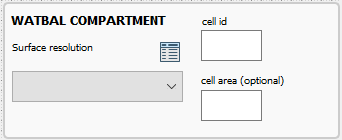
\includegraphics[
        width=0.8\linewidth
    ]{
        2_application_user_guide/fig/DialogSelectLayer_watbal.png
    }} \captionof{figure}{WATBAL compartment configuration fields}
\end{minipage}

\vspace{1em}
\textbf{The hydraulic compartment (\gui{HYD COMPARTMENT})}

\begin{minipage}[t]{0.45\textwidth}
    \begin{itemize}
        \item \gui{Hyd resolution}: name of the output resolution of the \gui{HYD} compartment (river elements);
        \item \gui{GIS Id}: the column number in the attribute table corresponding to the GIS identifier of the cells
    \end{itemize}
\end{minipage}%
\hfill
\begin{minipage}[t]{0.45\textwidth}
    \centering
    \raisebox{\dimexpr-\height+\ht\strutbox}{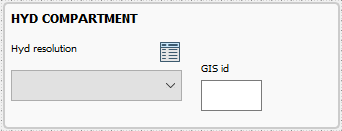
\includegraphics[
        width=0.8\linewidth
    ]{
    2_application_user_guide/fig/DialogSelectLayer_hyd.png
    }}
    \captionof{figure}{HYD compartment configuration fields}
\end{minipage}

\vspace{1em}
\textbf{The unsaturated compartment (\gui{NSAT COMPARTMENT}):}

\begin{minipage}[t]{0.45\textwidth}
    \begin{itemize}
        \item \gui{Unsatured zone resolution}: name of the output resolution of the \gui{NSAT} compartment;
        \item \gui{cell id}: the column number in the attribute table corresponding to the cell identifier.
    \end{itemize}
\end{minipage}%
\hfill
\begin{minipage}[t]{0.45\textwidth}
    \centering
    \raisebox{\dimexpr-\height+\ht\strutbox}{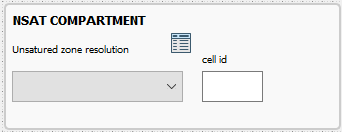
\includegraphics[
        width=0.8\linewidth
    ]{
    2_application_user_guide/fig/DialogSelectLayer_nsat.png
    }}
    \captionof{figure}{NSAT compartment configuration fields}
\end{minipage}

\vspace{1em}
\textbf{The saturated compartment (\gui{AQ COMPARTMENT})}

\begin{minipage}[t]{0.45\textwidth}
     \begin{itemize}
            \item \gui{Aquiferes resolutions}: the GIS layers constituting the
                underground mesh. The selected layer is added by clicking
                on \gui{Add}. Layers must be ordered from the uppermost
                to the lowermost layer using the \gui{up} and \gui{down} buttons.
                Finally, a layer can be removed from the list by clicking on
                \gui{remove};
            \item \gui{cell id abs}: identifier of the attribute table column
                containing the absolute cell identifier. This identifier
                can be homogeneous across GIS layers: in that case, \gui{homogeneous ID ABS}
                must be selected. Otherwise, click on \gui{heterogeneous ID ABS}
                to open dialog boxes allowing you to specify, for
                each layer, the column containing the ABS ID of the cells (cf. Fig \ref{fig_id_abs_hetero}).
        \end{itemize}
\end{minipage}%
\hfill
\begin{minipage}[t]{0.45\textwidth}
    \centering
    \raisebox{\dimexpr-\height+\ht\strutbox}{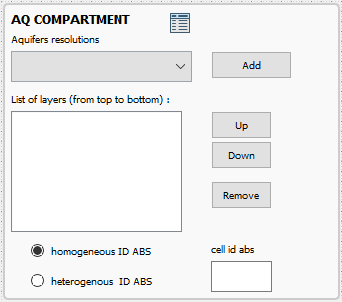
\includegraphics[
        width=0.8\linewidth
    ]{
    2_application_user_guide/fig/DialogSelectLayer_aq.png
    }}
    \captionof{figure}{AQ compartment configuration fields}
    \raisebox{\dimexpr-\height+\ht\strutbox}{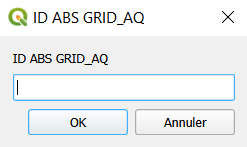
\includegraphics[
        width=0.5\linewidth
    ]{
2_application_user_guide/fig/DialogSelect_Layer_hetero_ID_ABS
    }}
    \label{fig_id_abs_hetero}
    \captionof{figure}{Window for selecting the field identifier containing the \gui{ID ABS} in the attribute table in the case of heterogeneous field identifiers across layers}
\end{minipage}



\alertwarning{Some points of caution:}
\begin{itemize}
    \item \textbf{The identifier of the first column of an attribute table starts at 0}. The icon 
\includegraphics[height=0.45cm]{2_application_user_guide/fig/table.png} allows viewing the identifiers of the fields listed in the attribute table of the resolution selected in the drop-down list;
    \item the code (e.g., BSS code) of an observation point must be \textbf{unique} among all observation points;
    \item The geometric configuration of the compartments checked in the project parameterisation dialog box must be defined in the geometry configuration dialog box.
\end{itemize}

\vspace{8pt}

\textbf{Extraction points - \gui{Hydrological and Hydrological plots}} \\
Extraction points can be of two types:
\begin{itemize}
    \item[$\bullet$] simple extraction points, which allow
    viewing simulated variables at those points;
    \item[$\bullet$] observation points, which allow comparing simulated variables with observation data at those points.
\end{itemize}



The configuration of extraction points requires specifying in the \gui{GIS Layer} fields the name of the layer in the QGIS project containing the observation points and extraction points according to the relevant \cws~compartment. The field identifiers to be specified are as follows:
\vspace{8pt}

\begin{minipage}[t]{0.45\textwidth}
    \textbf{Extraction points of the \gui{HYD} compartment}
    \vspace{4pt}

     \underline{Extraction points}

    \begin{itemize}
        \item \gui{name}: name of the observation point;
        \item \gui{ID GIS}: GIS identifier of the observation point to which the observation point must be attached (optional field)
    \end{itemize}

    \vspace{2pt}
    \underline{Observation points}
    \begin{itemize}
        \item \gui{code}: identification code of the observation point, must be unique for each point. The observation file for the point must have the same name with the \script{.dat} extension;
        \item the \gui{name} and \gui{ID GIS} fields are also specified for the configuration of observation points
    \end{itemize}
    \vspace{8pt}
    \textbf{Extraction points of the \gui{AQ} compartment}
    \vspace{4pt}

     \underline{Extraction points}

    \begin{itemize}
        \item \gui{name}: name of the observation point;
        \item \gui{ID LAYER}: identifier of the aquifer layer
        \item \gui{ID GIS}: GIS identifier of the observation point to which the observation point must be attached (optional field)
    \end{itemize}

    \vspace{2pt}
    \underline{Observation points}
    \begin{itemize}
        \item \gui{code}: identification code of the observation point, must be unique for each point. The observation file for the point must have the same name with the \script{.dat} extension;
        \item the \gui{name} and \gui{ID GIS} fields are also specified for the configuration of observation points
    \end{itemize}


\end{minipage}%
\hfill
\begin{minipage}[t]{0.45\textwidth}
    \centering
    \raisebox{\dimexpr-\height+\ht\strutbox}{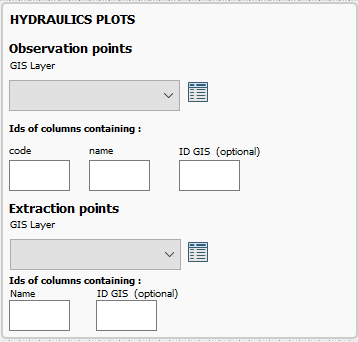
\includegraphics[
        width=0.9\linewidth
    ]{
    2_application_user_guide/fig/DialogSelectLayer_hyd_extraction.png
    }}
    \captionof{figure}{Configuration fields for \gui{HYD} compartment extraction points}
    \vspace{4pt}
    \raisebox{\dimexpr-\height+\ht\strutbox}{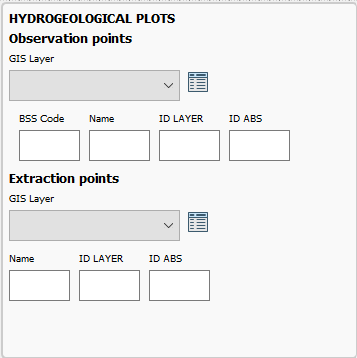
\includegraphics[
        width=0.9\linewidth
    ]{
    2_application_user_guide/fig/DialogSelectLayer_aq_extraction
    }}
    \label{fig_aq_extraction}
    \captionof{figure}{Configuration fields for \gui{AQ} compartment extraction points}
\end{minipage}

\alertwarning{
Extraction points must be contained in a \script{.shp} file different from the observation points. Points cannot be contained in the same file if they are extracted from two different compartments.
}


\alertinfo{
A preliminary save of the geometry configuration file can be saved by specifying a file path in the field located at the bottom left of the dialog box. This file (\cfcod \ref{code_config_geom}) will be saved upon execution of the \gui{Settings} dialog box if the configured project does not yet exist in the post-processing
directory specified.
Multiple project configurations can be saved in the same post-processing directory, provided they do not have the same project name. }



\section{Configuring Resolutions from a \json~Configuration File}

The geometric configuration of resolutions can be specified via a
\json~file according to the following structure:

\begin{lstlisting}[language=json, caption={Contents of a geometry configuration file}, label={code_config_geom}]
{   // list of CaWaQS compartments to analyse (1 = AQ, 2 = HYD, 3 = WATBAL)
    "ids_compartment": [],

    "resolutionNames":
    {
        "1":
            [[""]], // list of names of aquifer meshes in the QGIS project
        "2" :
            [[""]], // name of the river mesh in the QGIS project
        "3" :
            [[""]] // name of the surface mesh in the QGIS project
        "4" :
            [[""]] // name of the unsaturated zone mesh in the QGIS project
        },
    "ids_col_cell": { // "compartment id" : "column number of cell id"
        "1" : "",  // "AQ id" : "absolute id column number"
        "2" : "",  //"HYD id" : "GIS id column number"
        "3" : ""   // "WATBAL id" : "cell id column number"
        },
    "obsNames": {
    // "compartment id" : "name of associated obs shp in the QGIS project"
        "1": "",
        "2" : ""
        },
    "obsIdsColCells": {
    // "compartment id" : "field number of the measurement point code"
        "1": "",
        "2": ""
        },
    "obsIdsColNames": {
    // "compartment id" : "field number of the measurement point name"
        "1": "",
        "2" : ""
        },
    "obsIdsColLayers": {
    // "compartment id" : "field number of the aquifer layer identifier"
        "1": "",
        "2" : null
        },
    "obsIdsCell": {
    // "comp. id" : "field number of the absolute or gis id of cell attached to obs"
        "1" : "",
        "2" : null
    },
     "extNames": {
    // "compartment id" : "name of associated extraction shp in the QGIS project"
        "2": "",
        "1": ""
    },
    "extIdsColNames": {
    // "compartment id" : "field number containing the extraction point name"
        "2": "",
        "1": ""
    },
    "extIdsColLayers": {
    // "compartment id" : "field number containing the aquifer layer identifier"
        "2": null,
        "1": ""
    },
    "extIdsColCells": {
    // "compartment id" : "field number containing the cell identifier"
        "1": "",
        "2": "",
    }
}
}
\end{lstlisting}
